\documentclass[a4paper,11pt]{article}

% Language setting
\usepackage[english]{babel}

% Font and encoding - Good practice for PDF output
\usepackage[T1]{fontenc}
\usepackage{lmodern}

% Page size and margins
\usepackage[top=2cm,bottom=2cm,left=2.2cm,right=2.2cm,marginparwidth=1.75cm]{geometry}

% Useful packages
\usepackage{amsmath}
\usepackage{graphicx}
\usepackage{float} % Keep float for [H] or [htbp]
\usepackage[hidelinks]{hyperref} % Hidelinks removes the colored boxes
\hypersetup{colorlinks=true,allcolors=blue}

% Packages for better tables
\usepackage{booktabs} % For professional tables (\toprule, \midrule, \bottomrule)
\usepackage{array} % For table column formatting

% Package for diagrams
\usepackage{tikz}
\usetikzlibrary{shapes,arrows,positioning}

% Graphics path (images folder is at repo root, one level up from 'rapport')
\graphicspath{{../images/}}

% Title
\title{Simple Consensus System for Distributed Locks\\
\large ICT3 Project n°2 — Shanghai Jiao Tong University}
\author{Alexandra Baron \and Charles Pelong \and Maria Stivala \and Arnaud Brisset \and Baptiste Halçaren \and Mathis Liens}
\date{October 2025}

\begin{document}

\maketitle

% University logo - Placed AFTER title and smaller
\begin{figure}[htbp]
\centering

\includegraphics[width=0.6\linewidth]{shanghai-jiao-tong-university.png}
\end{figure}

\begin{abstract}
This report presents the design and implementation of a simple consensus system for managing distributed locks using a leader-follower architecture. The implementation, realized in \texttt{Java} using sockets, guarantees strong consistency: all mutation operations (\emph{lock}/\emph{unlock}) are validated by the leader and then replicated to all followers, while read requests (\emph{own}) are served locally by any server. We describe the project's objective, the methodology used, the system architecture, and the code structure. Finally, we present experimental results and discuss the system's limitations.
\end{abstract}

\section{Context and Objective}
As part of the ICT3 (Information and Communication Technologies) course, the objective was to \textbf{design a simple consensus system} meeting the following requirements: (i) one leader and multiple followers; (ii) a replicated \textit{map} (key $\rightarrow$ owner) for the locks; (iii) multiple clients able to \texttt{tryLock}, \texttt{tryUnLock}, and \texttt{ownTheLock}; (iv) \textbf{all} mutation operations (\texttt{LOCK}/\texttt{UNLOCK}) must be routed to the leader; (v) read operations (\texttt{OWN}) can be served locally by followers; (vi) the leader updates its map and \textbf{propagates an update proposal} to all followers.

The core challenge is ensuring data consistency, guaranteeing that all servers have the same view of who owns which lock, especially during concurrent client requests.

\section{Method and Implementation Choices}
We opted for a \textbf{leader-follower architecture} built on Java TCP sockets. This approach was chosen for its explicit control over the network communication and its suitability for the project's requirements.

\begin{itemize}
    \item \textbf{Reasoning (Technology Choice)}: Java was selected as suggested in the project subject. Its built-in socket libraries (\texttt{java.net}) and robust concurrency utilities (\texttt{java.util.concurrent}) are well-suited for this task. The \texttt{ExecutorService} provides an efficient way to manage client connections without the overhead of creating a new thread for every request.

    \item \textbf{Minimalist Text Protocol}: We designed a simple, human-readable text protocol (e.g., \texttt{LOCK,<lockName>,<clientId>}). This choice simplifies debugging and implementation compared to a binary protocol, which would require more complex serialization/deserialization logic.

    \item \textbf{Request Routing}: Followers act as simple routers for write operations, forwarding \texttt{LOCK}/\texttt{UNLOCK} requests to the leader. This design decision is central to ensuring consistency, as it establishes the leader as the single point of truth (or "single-writer") for all state changes, preventing split-brain scenarios.

    \item \textbf{Pending Request Mechanism}: Following the project specifications, when a follower receives a \texttt{LOCK} or \texttt{UNLOCK} request, it marks the request as \emph{pending} and keeps the client connection open. The follower forwards the request to the leader. If the leader returns \texttt{FAIL}, the follower responds immediately. If the leader returns \texttt{SUCCESS}, the follower waits for the \texttt{SYNC} message. When the \texttt{SYNC} arrives, the follower updates its local map, checks if the request is pending, and if so, sends the \texttt{SUCCESS} response to the client. This mechanism ensures that clients receive confirmation only after the state change has been replicated via the \texttt{SYNC} message.
    
    \item \textbf{Synchronous Replication}: The leader uses a synchronous \texttt{SYNC}/\texttt{ACK} model for replication. When the leader approves a \texttt{LOCK} or \texttt{UNLOCK} operation, it updates its local map and sends a \texttt{SYNC} message to all followers in parallel (using a thread pool). The leader then \textbf{waits for ACK from all followers} using a \texttt{CountDownLatch} before considering the replication complete. This ensures that when the leader returns \texttt{SUCCESS} (either directly to a client or to a follower that forwarded the request), all followers have received and acknowledged the state change. The follower that forwarded the request also waits for the \texttt{SYNC} before responding to its client, providing strong consistency guarantees.
    
    \item \textbf{Reasoning (Consistency)}: The synchronous replication combined with the pending request mechanism provides strong consistency: when a client receives a \texttt{SUCCESS} response from a follower, it has a guarantee that the state change has been (1) accepted by the leader, (2) replicated to \textbf{all followers} (via synchronous SYNC/ACK), and (3) applied to that specific follower's map. This ensures that all servers in the cluster have a consistent view of the lock state before any client receives confirmation of a successful operation. The synchronous approach trades some latency for strong consistency guarantees, which is appropriate for a distributed lock system.

    \item \textbf{Simple Error Handling}: The system relies on socket timeouts (5-10s) and explicit response codes (\texttt{SUCCESS}/\texttt{FAIL}/\texttt{NONE}/\texttt{ERROR}/\texttt{TIMEOUT}). This provides basic robustness against network delays or unresponsive servers without implementing a complex failure-detection and leader-election protocol, which was deemed outside the project's scope.
\end{itemize}

\section{Data Flow and Architecture}
The system's functional architecture is centralized around the leader, which serializes all state changes. The interactions are as follows:

\begin{enumerate}
    \item \textbf{Write Operation (LOCK/UNLOCK)}: 
    \begin{itemize}
        \item \textbf{From Follower}: Client $\rightarrow$ Follower (marks request as \emph{pending}, keeps connection open) $\rightarrow$ Follower forwards request to Leader asynchronously $\rightarrow$ Leader processes, updates map, sends \texttt{SYNC} to all followers (including the one that forwarded), and waits for all \texttt{ACK} (synchronous replication) $\rightarrow$ Leader responds \texttt{SUCCESS} to follower's forwarding thread, but the follower ignores this response and waits for \texttt{SYNC} $\rightarrow$ Follower receives \texttt{SYNC}, updates local map, checks if request is \emph{pending}, sends \texttt{ACK} to leader, and if request is pending, sends \texttt{SUCCESS} to client and closes connection. If the leader returns \texttt{FAIL} (before sending SYNC), the follower responds immediately to client and closes connection.
        \item \textbf{From Leader}: Client $\rightarrow$ Leader $\rightarrow$ Leader processes, updates map, sends \texttt{SYNC} to all followers, waits for all \texttt{ACK} (synchronous replication), then responds \texttt{SUCCESS} to client.
    \end{itemize}
    \item \textbf{Read Operation (OWN)}: Client $\rightarrow$ (Any) Server $\rightarrow$ Client. This operation is handled locally by whichever server receives it to ensure low latency. The response is sent immediately and the connection is closed.
    \item \textbf{Follower Registration}: When a follower server starts, it sends a \texttt{REGISTER,\$ip:\$port} message to the leader. The leader adds the follower to its internal list and responds with \texttt{REGISTERED}. This allows the leader to know which followers to notify during replication.
\end{enumerate}

This flow is illustrated in Figure \ref{fig:mermaid}, which shows the sequence of network calls for both a write (\texttt{LOCK}) and a read (\texttt{OWN}) operation.

% Note: This figure requires you to export your Mermaid diagram to "images/mermaid-flow.png"
\begin{figure}[htbp]
    \centering
    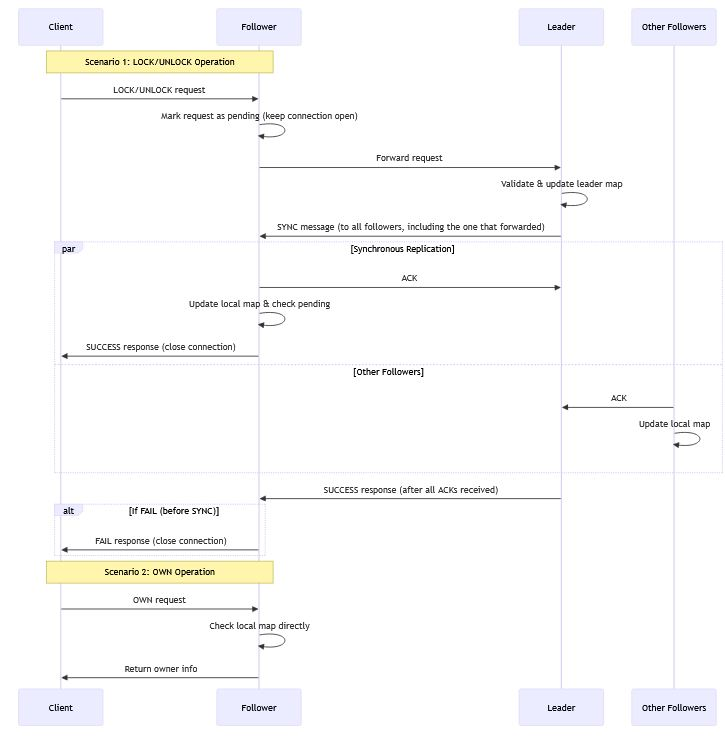
\includegraphics[width=0.85\linewidth]{images/capture_architecture_from_readme.JPG}
    \caption{Sequence diagram of system operations (LOCK and OWN).}
    \label{fig:mermaid}
\end{figure}

\newpage
\section{Structure of the Code}
The project consists of three main Java classes:

\begin{itemize}
    \item \textbf{\texttt{Client.java}}: This class provides the client-facing API: \texttt{tryLock}, \texttt{tryUnLock}, and \texttt{ownTheLock}. Each operation opens a new, short-lived socket, sends its request message via \texttt{sendMsg()}, and reads the single-line response from the server.

    \item \textbf{\texttt{DistributedLockTest.java}}: A test suite that uses a \texttt{FixedThreadPool} to simulate concurrent clients. These clients connect to different servers in the cluster (the leader at 10.0.2.3, and followers at 10.0.2.4 / 10.0.2.5) to verify concurrent lock acquisition, owner-reading, and lock release.
    
    \item \textbf{\texttt{Server.java}}: This is the core class, capable of running in either "leader" or "follower" mode. It uses a \texttt{CachedThreadPool} to handle each incoming connection in a separate thread (\texttt{handleClient()}).
        \begin{itemize}
            \item \texttt{handleClientRequest()}: Parses client messages (\texttt{LOCK}, \texttt{UNLOCK}, \texttt{OWN}) and handles them according to the server role. For \texttt{OWN} requests, it responds immediately. For \texttt{LOCK}/\texttt{UNLOCK} on a leader, it processes and responds immediately. For \texttt{LOCK}/\texttt{UNLOCK} on a follower, it implements the \emph{pending request} mechanism (see below).
            \item \texttt{processRequest()}: This \texttt{synchronized} method is the main logic gate for business rule enforcement.
                \begin{itemize}
                    \item If \textbf{isLeader}, it calls \texttt{handleLeaderRequest()} to enforce business rules, update the local \texttt{lockMap}, and trigger replication via \texttt{notifyFollowers()}.
                    \item If \textbf{isFollower}, it calls \texttt{handleFollowerRequest()} (only used for \texttt{OWN} requests in the pending implementation).
                \end{itemize}
            \item \textbf{Pending Request Mechanism} (for LOCK/UNLOCK on followers): When a follower receives a \texttt{LOCK} or \texttt{UNLOCK} request:
                \begin{itemize}
                    \item The request is marked as \emph{pending} (stored in \texttt{pendingRequests} map with key \texttt{lockName:clientId:cmd}) and the client connection is kept open.
                    \item The request is forwarded to the leader in a separate thread via \texttt{forwardToLeaderForPending()} (non-blocking for the main connection handler).
                    \item If the leader returns \texttt{FAIL}, the follower responds immediately to the client and closes the connection.
                    \item If the leader returns \texttt{SUCCESS}, the follower waits for the \texttt{SYNC} message.
                \end{itemize}
            \item \texttt{handleSyncMessage()} and \texttt{processSync()}: When a follower receives a \texttt{SYNC} message, \texttt{handleSyncMessage()} is called, which then invokes \texttt{processSync()}. This method:
                \begin{itemize}
                    \item Updates the local \texttt{lockMap} according to the SYNC command.
                    \item Checks if the request is \emph{pending} (by constructing the pending key from the SYNC parameters).
                    \item If the request is pending, sends \texttt{SUCCESS} response to the client and closes the connection.
                \end{itemize}
                After \texttt{processSync()} completes, \texttt{handleSyncMessage()} sends the \texttt{ACK} back to the leader.
            \item \texttt{notifyFollowers()}: The leader iterates through its list of followers, submitting a new task to the thread pool for each one to send a \texttt{SYNC} message in parallel. The leader uses a \texttt{CountDownLatch} to synchronously wait for \texttt{ACK} responses from all followers. This ensures that the leader does not return \texttt{SUCCESS} until all followers have received and acknowledged the state change, providing synchronous replication and strong consistency guarantees. Each task has a 5-second timeout, and the leader has a 10-second overall timeout for all ACKs.
        \end{itemize}
\end{itemize}

\subsection*{Business Rules (Enforced by Leader)}
\begin{itemize}
    \item \textbf{Preemption (LOCK)}: Success if the lock (key) does not exist in the \texttt{lockMap}. Failure otherwise.
    \item \textbf{Release (UNLOCK)}: Success if the lock (key) exists *and* the caller's \texttt{clientId} matches the one stored in the map. Failure otherwise.
    \item \textbf{Read (OWN)}: Any client can query the owner. The request is handled by any server and returns the owner's \texttt{clientId} or \texttt{NONE} if the lock does not exist.
\end{itemize}

\section{Communication Protocol and Error Handling}
The system uses a simple, text-based, comma-delimited protocol.

\subsection*{Client-Server Messages}
\begin{table}[htbp]
\centering
\caption{Client-Server and Inter-Server Protocol}
\label{tab:protocol}
\begin{tabular}{@{}lll@{}}
\toprule
\textbf{Type} & \textbf{Format} & \textbf{Description} \\
\midrule
Client $\rightarrow$ Server & \texttt{LOCK,\$name,\$client} & Lock acquisition request \\
Client $\rightarrow$ Server & \texttt{UNLOCK,\$name,\$client} & Lock release request \\
Client $\rightarrow$ Server & \texttt{OWN,\$name,\$client} & Read owner request \\
Leader $\rightarrow$ Followers & \texttt{SYNC,\$cmd,\$name,\$client} & State replication (e.g., SYNC,LOCK,...) \\
Followers $\rightarrow$ Leader & \texttt{ACK} & Acknowledgment of SYNC \\
Followers $\rightarrow$ Leader & \texttt{REGISTER,\$ip:\$port} & Follower registration on startup \\
Leader $\rightarrow$ Follower & \texttt{REGISTERED} & Confirmation of successful registration \\
Leader $\rightarrow$ Follower & \texttt{NOT\_LEADER} & Response when non-leader receives REGISTER \\
\bottomrule
\end{tabular}
\end{table}

\subsection*{Server Responses and Error Handling}
Server responses to the client are simple, single-word strings, as shown in Table \ref{tab:responses}. This provides basic robustness. Timeouts are implemented on socket operations to prevent threads from hanging indefinitely on network issues: 30 seconds for pending client connections (to allow time for SYNC to arrive), 10 seconds for forwarding requests to the leader, 5 seconds per follower for SYNC operations, and a 10-second overall timeout for receiving all ACKs during replication.

\begin{table}[htbp]
\centering
\caption{Server Response Codes}
\label{tab:responses}
\begin{tabular}{@{}ll@{}}
\toprule
\textbf{Response Code} & \textbf{Meaning} \\
\midrule
\texttt{SUCCESS} & Operation (LOCK/UNLOCK) succeeded. \\
\texttt{FAIL} & Operation (LOCK/UNLOCK) failed (e.g., lock taken, not owner). \\
\texttt{NONE} & \texttt{OWN} request returned no owner for the lock. \\
\texttt{<ClientID>} & \texttt{OWN} request returned the current lock owner. \\
\texttt{ERROR} & A generic connection or processing error occurred. \\
\texttt{TIMEOUT} & A network operation (e.g., forwarding) timed out. \\
\texttt{INVALID\_FORMAT} & Message format is invalid (not enough parts). \\
\texttt{INVALID\_COMMAND} & Command type is not recognized (not LOCK/UNLOCK/OWN). \\
\bottomrule
\end{tabular}
\end{table}

\textbf{Note}: Additional inter-server response codes include \texttt{REGISTERED} and \texttt{NOT\_LEADER}, used during follower registration with the leader.

\section{Experimental Results}
The following figures illustrate the system in operation, using three virtual machines as specified in the \texttt{README.md}.

\begin{figure}[H]
\centering
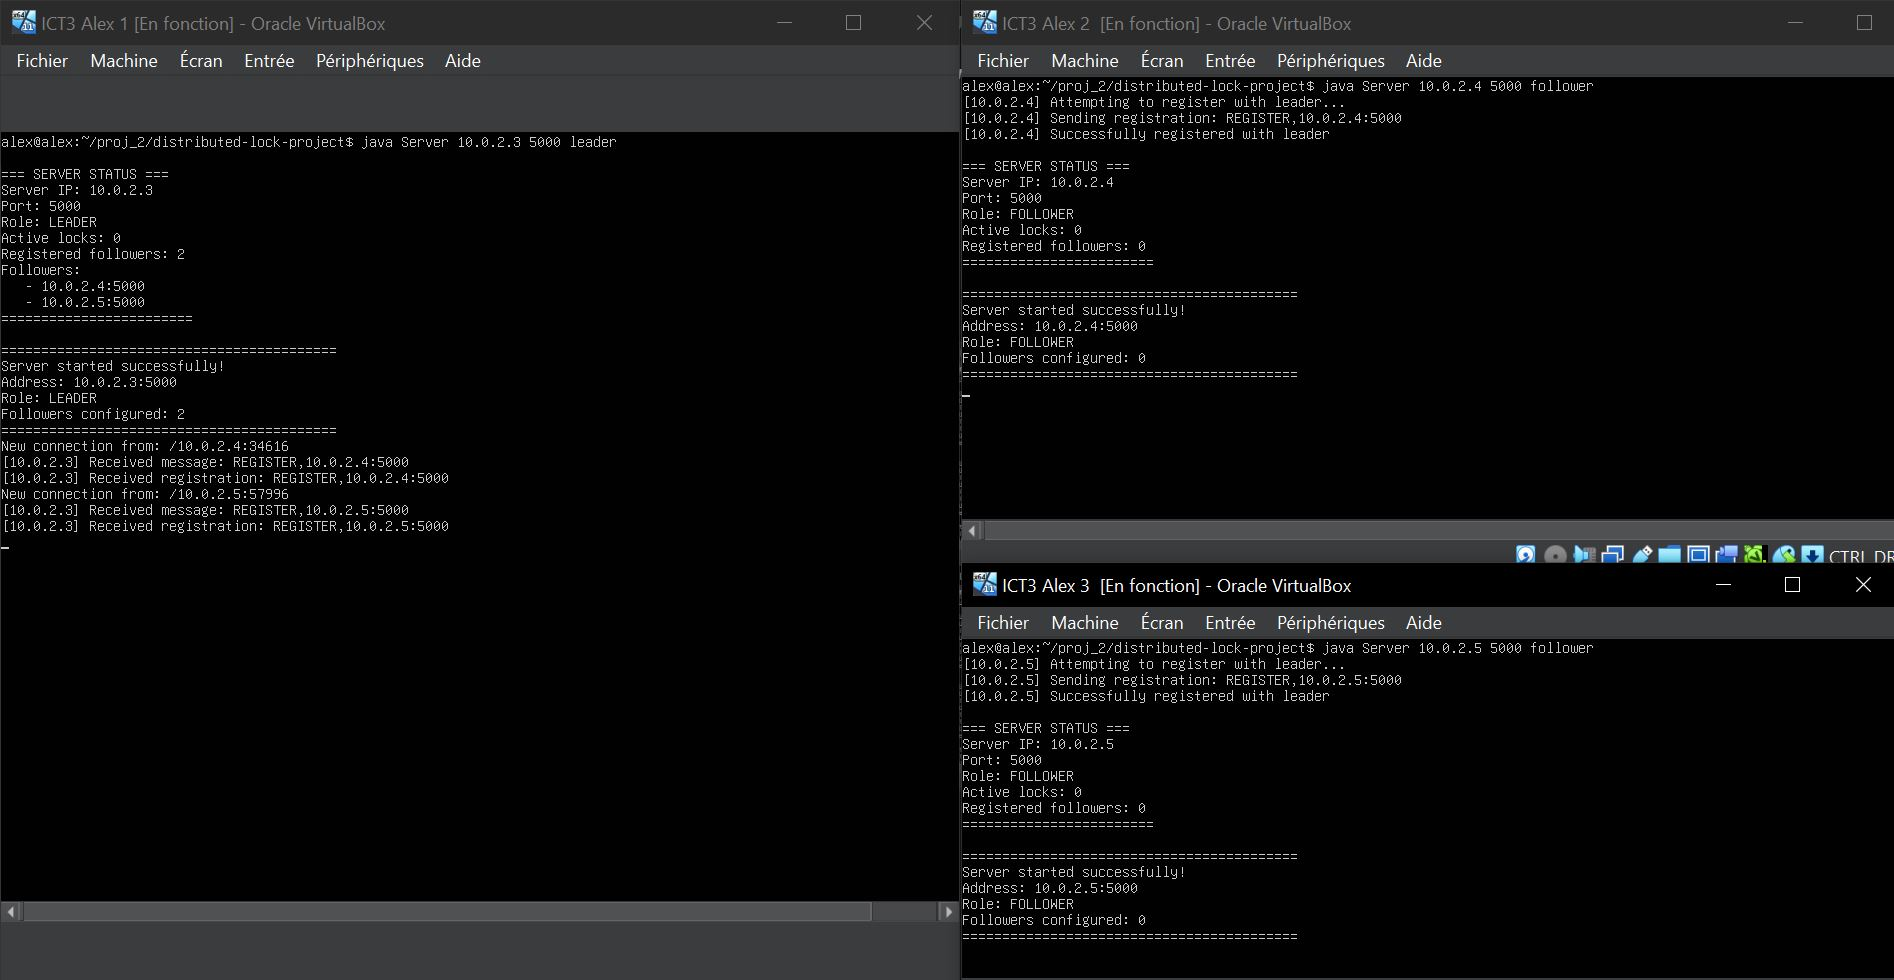
\includegraphics[width=1\linewidth]{images/Capture_connection des 3 serveurs .JPG}
\caption{Initialization of the leader (10.0.2.3) and the two followers (10.0.2.4, 10.0.2.5).}
\end{figure}

\begin{figure}[H]
\centering
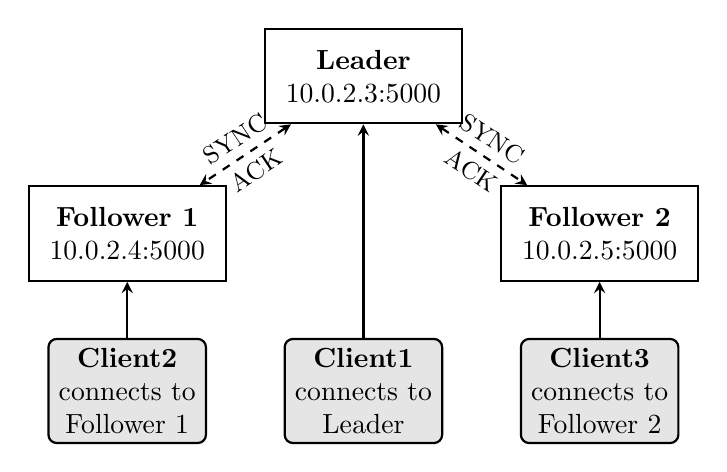
\begin{tikzpicture}[
    node distance=1.5cm and 2cm,
    server/.style={rectangle, draw, thick, minimum width=2.5cm, minimum height=1.2cm, align=center},
    client/.style={rectangle, draw, thick, rounded corners=3pt, minimum width=2cm, minimum height=1cm, align=center, fill=gray!20},
    connection/.style={->, >=stealth, thick}
]

% Servers
\node[server] (leader) at (0,4) {\textbf{Leader}\\10.0.2.3:5000};
\node[server] (follower1) at (-3,2) {\textbf{Follower 1}\\10.0.2.4:5000};
\node[server] (follower2) at (3,2) {\textbf{Follower 2}\\10.0.2.5:5000};

% Clients (Client1 et Client2 échangés)
\node[client] (client2) at (-3,0) {\textbf{Client2}\\connects to\\Follower 1};
\node[client] (client1) at (0,0) {\textbf{Client1}\\connects to\\Leader};
\node[client] (client3) at (3,0) {\textbf{Client3}\\connects to\\Follower 2};

% Client to Server connections
\draw[connection] (client1) -- (leader);
\draw[connection] (client2) -- (follower1);
\draw[connection] (client3) -- (follower2);

% Inter-server connections (SYNC/ACK) - flèches double sens
% Leader <-> Follower 1
\draw[connection, dashed, <->] (leader) -- node[midway, above, sloped, font=\small] {SYNC} node[midway, below, sloped, font=\small] {ACK} (follower1);
% Leader <-> Follower 2
\draw[connection, dashed, <->] (leader) -- node[midway, above, sloped, font=\small] {SYNC} node[midway, below, sloped, font=\small] {ACK} (follower2);

\end{tikzpicture}
\caption{Test architecture for \texttt{DistributedLockTest}: three clients connect to different servers (Client1 to the leader, Client2 and Client3 to the followers) to test concurrent lock operations and replication.}
\label{fig:test_architecture}
\end{figure}

\begin{figure}[H]
\centering
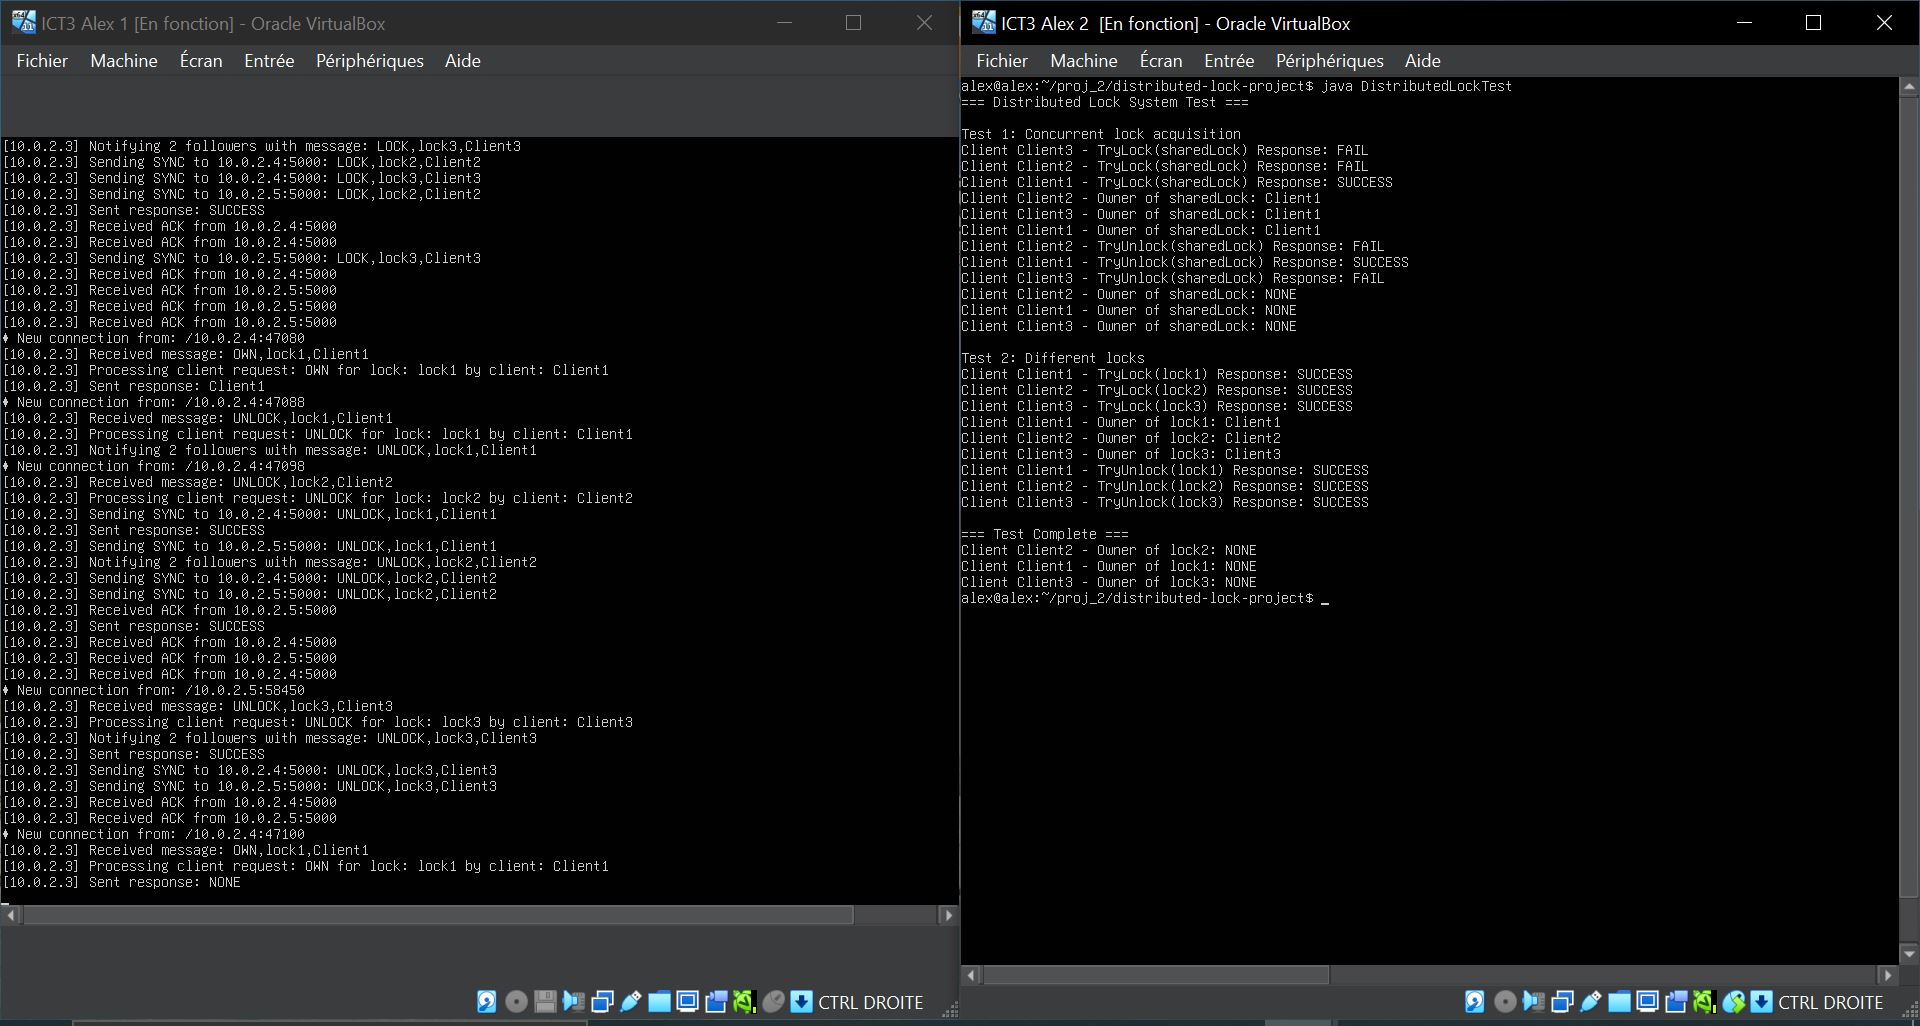
\includegraphics[width=1\linewidth]{images/Capture_distributed_lock_test.JPG}
\caption{Execution of \texttt{DistributedLockTest}: concurrent acquisitions, reads, and releases. The test architecture is shown in Figure \ref{fig:test_architecture}.}
\end{figure}


\subsection*{Observations}
\begin{itemize}
    \item The test results show that for a single lock, only one client's \texttt{LOCK} request succeeds, while concurrent attempts from other clients correctly fail (returning \texttt{FAIL}). The architecture shown in Figure \ref{fig:test_architecture} demonstrates how the three clients connect to different servers in the cluster.
    \item \texttt{OWN} requests, even when sent to followers, correctly return the ID of the lock owner or \texttt{NONE} after the lock is released. Due to the synchronous replication mechanism, followers should always have the most up-to-date data, ensuring strong consistency across all servers.
    \item The \texttt{SYNC} replication mechanism successfully maintains strong consistency across the leader and all followers. The synchronous replication (with ACK confirmation) ensures that all state changes are replicated to all followers before any client receives confirmation, guaranteeing a consistent view across the entire cluster.
\end{itemize}

\section{Limitations and Future Work}
While functional, this implementation has several limitations that could be addressed in future work.
\begin{itemize}
    \item \textbf{Hard-coded Configuration}: The leader's address (10.0.2.3) and the list of followers are hard-coded in \texttt{Server.java}. This is inflexible. A better solution would use a configuration file or command-line arguments to define the cluster topology.
    \item \textbf{Fault Tolerance}: The system has a single point of failure (SPOF): the leader. If the leader server crashes, the system can no longer process any \texttt{LOCK} or \texttt{UNLOCK} requests. A robust system would require a fault-tolerance mechanism, such as leader election (e.g., using Paxos or Raft), which was outside the scope of this project. Additionally, if a follower fails during replication, the leader logs the error but continues, potentially leaving that follower out of sync until it recovers and re-registers.
    \item \textbf{Network}: Communication is unencrypted (plaintext), and there is no client authentication. This is insecure for a production environment.
    \item \textbf{Connection Management}: The pending request mechanism keeps client connections open while waiting for SYNC messages. While a 30-second timeout prevents indefinite hanging, this approach could be improved with connection pooling or more sophisticated connection lifecycle management for high-throughput scenarios.
    \item \textbf{Thread Safety}: While \texttt{ConcurrentHashMap} and synchronized methods provide thread safety, the combination of pending requests and synchronous replication could be further optimized to reduce contention under high load.
\end{itemize}

\section{Conclusion}
We have successfully implemented a distributed lock system that fulfills the core requirements of the project. It uses a leader-follower architecture with a simple Java socket protocol to manage \texttt{LOCK}, \texttt{UNLOCK}, and \texttt{OWN} operations. The system ensures strong consistency by routing all write operations through the leader and using synchronous replication (with pending request mechanism) to update followers. The leader waits for acknowledgments from all followers before confirming successful operations, ensuring that all servers maintain a consistent view of the lock state. The pending request mechanism further strengthens consistency by ensuring that clients receive confirmation only after their request has been replicated to the follower that processed it. Tests demonstrate the system's correctness in handling concurrent requests and maintaining a consistent state across all servers. This project serves as a solid foundation for understanding consensus and distributed system.

\end{document}
